\documentclass[12pt,a4paper]{ctexart}
\usepackage[margin=2.5cm]{geometry}
\usepackage{graphicx}
\usepackage{float}
\usepackage{booktabs}
\usepackage{xcolor}
\usepackage{hyperref}
\hypersetup{colorlinks=true, linkcolor=blue, urlcolor=blue}

\title{\textbf{文档一：微信公众号注册说明}\\[0.3em]
       \large Offer Show 微信公众号后台系统作业}
\author{顾远（YoungJude）\\北京交通大学 \quad API设计与实现}
\date{\today}

\begin{document}
\maketitle

\section{公众号基本信息}

本人已完成实名认证的个人微信公众号注册，相关信息如下表所示。

\begin{table}[H]
  \centering
  \begin{tabular}{ll}
    \toprule
    \textbf{项目} & \textbf{内容} \\
    \midrule
    公众号名称   & YoungJude \\
    类型         & 订阅号（公众号） \\
    简介         & hahahaha \\
    所在地区     & 中国\,北京\,朝阳 \\
    认证情况     & 未认证 \\
    主体信息     & 顾远（个人） \\
    总用户数     & 1 \\
    \bottomrule
  \end{tabular}
  \caption{微信公众号 YoungJude 的基本信息}
\end{table}

\section{公众号设置页截图}

下图为微信公众平台中本公众号的「账号详情」页面，展示了名称、类型、
简介、地区及主体信息等关键字段，可证明该公众号为本人实名注册。

\begin{figure}[H]
  \centering
  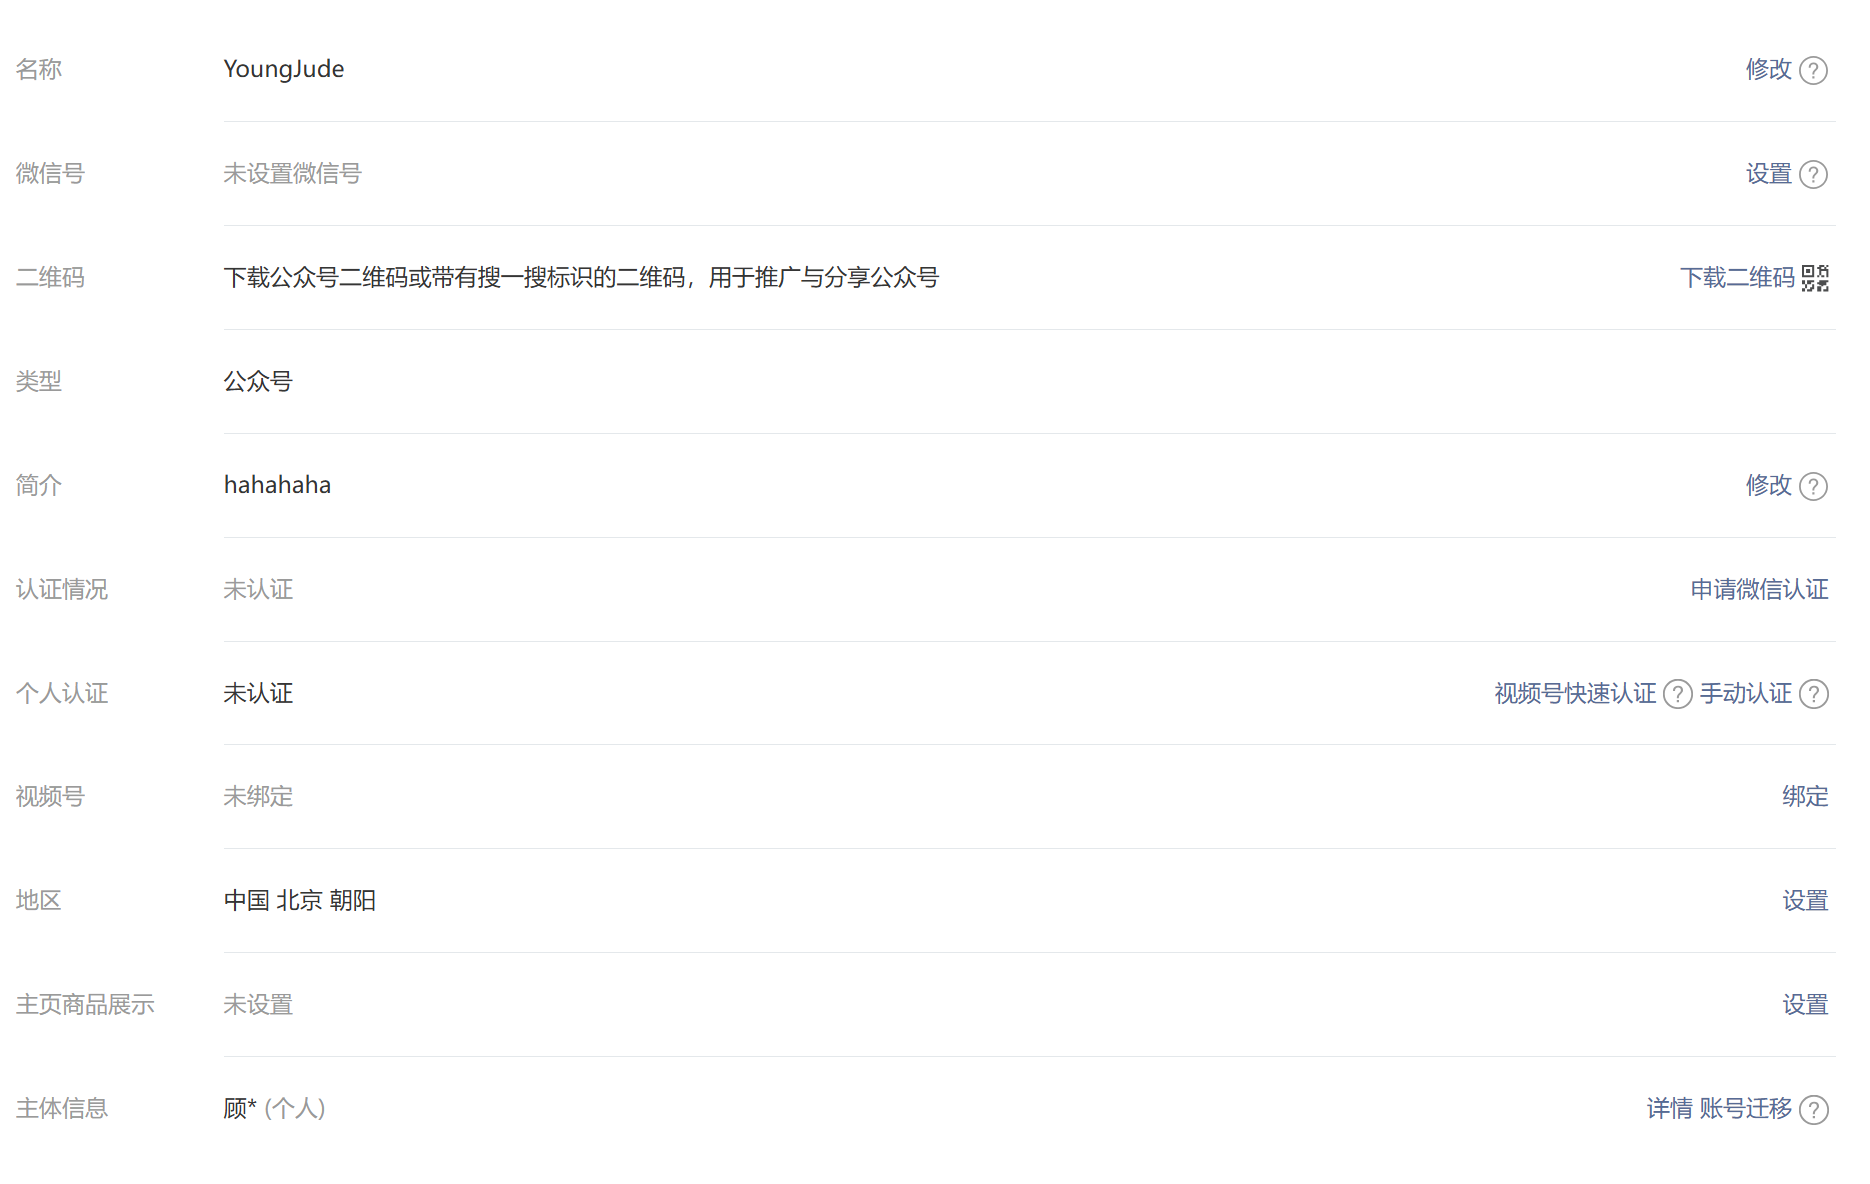
\includegraphics[width=\linewidth]{1.png}
  \caption{公众号账号详情页（YoungJude）}
\end{figure}

\section{公众号后台首页截图}

下图为微信公众平台后台首页，左侧为内容管理、互动管理、数据分析、
收入变现、广告与服务等功能入口，右侧展示昨日阅读数、分享数、
新增关注数及近期发表等运营数据。

\begin{figure}[H]
  \centering
  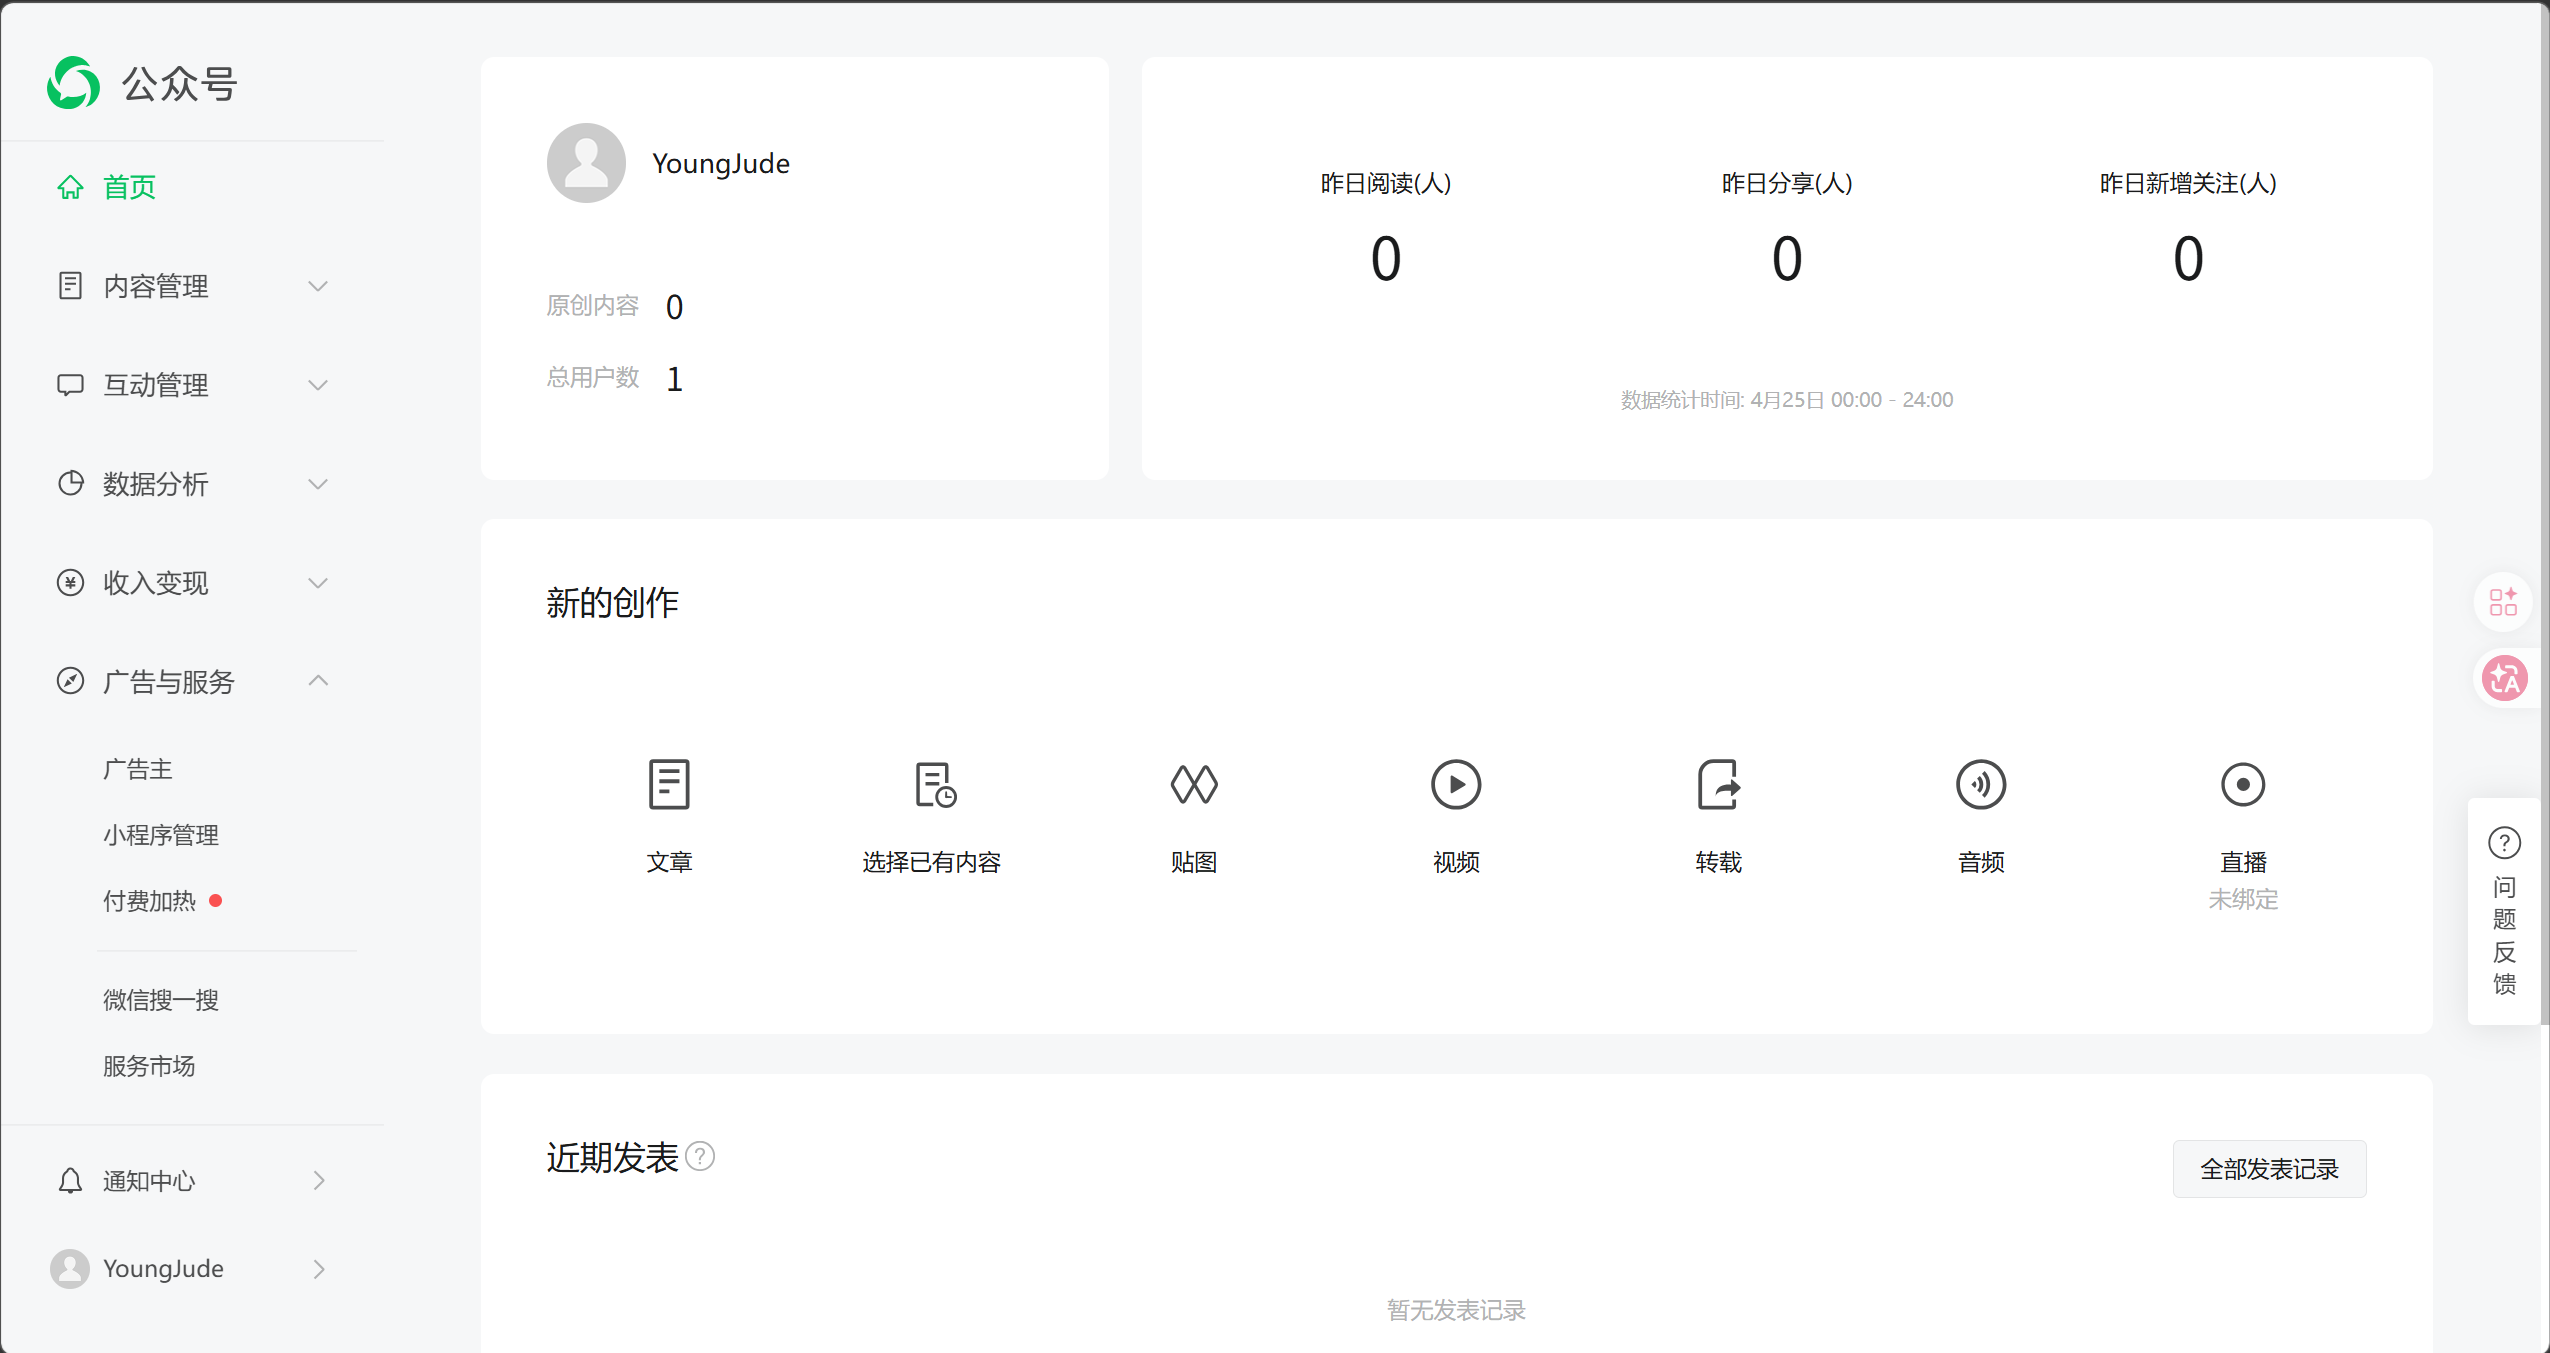
\includegraphics[width=\linewidth]{2.png}
  \caption{公众号后台首页（YoungJude）}
\end{figure}

\section{说明}

本公众号将作为后续作业「Offer Show 微信公众号后台系统」的对外交互入口，
通过该公众号接收用户消息并调用后台 API，完成名企实习校招信息检索、
薪资查询等功能的演示。

\end{document}
